\documentclass[12pt]{article}
\usepackage{amsmath, amssymb, amsthm}
\usepackage{import}
\usepackage{pdfpages}
\usepackage{transparent}
\usepackage{xcolor}
\usepackage{graphicx, epstopdf}

\usepackage{fancyhdr}
\usepackage[framed, numbered]{matlab-prettifier}

\fancyhf{}
\pagestyle{fancy}
\lhead{Carrera}
\rhead{\thepage}

\setlength\parindent{0pt}
\numberwithin{equation}{subsection}

\usepackage{titlesec}
\titleformat{\section}
{\normalfont\Large\bfseries}{Exercise~\thesection}{1em}{}

\newcommand{\incfig}[2][1]{%
  \def\svgwidth{#1\columnwidth}
  \import{./figures/}{#2.pdf_tex}
}

\newcommand{\RE}{\mathrm{Re}}
\newcommand{\IM}{\mathrm{Im}}

\newcommand\ddfrac[2]{\frac{\displaystyle #1}{\displaystyle #2}}

\pdfsuppresswarningpagegroup=1

\author{Adam Carrera}
\date{February 24 , 2021}
\title{MECH 3340 - Assignment \#4}

\begin{document}
  \maketitle

  \section{}

  \subsection{Part A}

  Given,

  \[
      A_c = 20 m^2, \quad \rho = 1000 kg/m^3, \quad h_0 = 5m, \quad R = 24.525 m^{-1}s^{-1}
    .\]

  We can form the system using conservation laws,

  \begin{equation}
    \frac{dm}{dt} = q_{mi} - q_{mo}
  \end{equation}

  where,

  \begin{equation}
    q_{mo} = \frac{\rho g}{R}h, \quad \frac{dm}{dt} = \rho A \dot h
  \end{equation}

  This gives us,

  \begin{equation}
    \rho A \dot h = q_{mi} - \frac{\rho g}{R}h
  \end{equation}

  \begin{equation}
    RC \dot h + h = \frac{R}{\rho g}q_{mi}
  \end{equation}

  where,

  \begin{equation}
    C = \frac{A}{g}
  \end{equation}

  Finally, we can calculate the time constant,

  \begin{equation}
    \tau = RC = 24.525 \times \frac{20}{9.8} = 50.051 \text{ seconds}
  \end{equation}

  \subsection{Part B}

  Find the height after 98\% of the water has left,

  General form,

  \begin{equation}
    \tau \dot x + x = k f(t)
  \end{equation}

  where,

  \begin{equation}
    f(t) = 0, \quad h(0) = 5m
  \end{equation}

  For free response, we have,

  \begin{equation}
    h(t) = h_0 e^{-\frac{1}{\tau}t}
  \end{equation}

  Clearly, $ h_\infty = 0 $ this means that,

  \begin{equation}
    \Delta h = h_0 - h_\infty = 5m
  \end{equation}

  \begin{equation}
    h_0 - 0.98\Delta h = 0.1m
  \end{equation}

  $ h = 0.1m $ when $ t = 195.801 = 7.95\tau. $ Therefore, 98\% of the water will have left the tank after 7.95 time constants.

  \subsection{Part C}

  We have,

  \begin{equation}
    RC \dot h + h = \frac{R}{\rho g}q_{mi}
  \end{equation}

  If water steadily flows in at a rate of 3000 kg/s, this means that the system is being subjected to a unit step response times 3000. Therefore, the steady state value will be

  \begin{equation}
    h_{ss} = 3000 * \frac{R}{\rho g} = 7.507m
  \end{equation}

  \section{}

  \subsection{Part A}


  We determine the system to be,

  \begin{equation}
    \begin{aligned}
      \rho A_1 \dot h_1 &= q_{mi} - \frac{\rho g}{R_1} (h_1 - h_2) \\
      \rho A_2 \dot h_2 &= \frac{\rho g}{R_1} (h_1 - h_2) - \frac{\rho g}{R_2}h_2
    \end{aligned}
  \end{equation}

  Move constants to RHS

  \begin{equation}
    \begin{aligned}
      \dot h_1 &= \frac{1}{\rho A_1}q_{mi} - \frac{g}{R_1 A_1}(h_1 - h_2) \\
      \dot h_2 &= \frac{g}{R_1 A_2} (h_1 - h_2) - \frac{g}{R_2 A_2}h_2
    \end{aligned}
  \end{equation}

  We can write the system in state space form, where $ h_1, \, h_2 $ are the state variables.

  \begin{equation}
    \begin{bmatrix}
      \dot h_1 \\ \dot h_2
    \end{bmatrix} =
    \begin{bmatrix}
      -\ddfrac{g}{R_1A_1} & \ddfrac{g}{R_1A_1} \\
      \ddfrac{g}{R_1A_2} & - \left( \ddfrac{g}{R_1A_2} + \ddfrac{g}{R_2A_2} \right)
    \end{bmatrix}
    \begin{bmatrix}
      h_1 \\ h_2
    \end{bmatrix} +
    \begin{bmatrix}
      \ddfrac{1}{\rho A_1} \\ 0
    \end{bmatrix} q_{mi}
  \end{equation}

  \begin{equation}
    y =
    \begin{bmatrix}
      0 & 1 \\
      0 & \ddfrac{\rho g}{R_2}
    \end{bmatrix}
    \begin{bmatrix}
      h_1 \\ h_2
    \end{bmatrix}
  \end{equation}

  \subsection{Part B}

  Substitue given values for $ R_1, R_2, A_1, A_2, \rho, g. $

  \begin{equation}
    \dot h =
    \begin{bmatrix}
      -1 & 1 \\
      \ddfrac{1}{4} & \ddfrac{1}{3}
    \end{bmatrix} h +
    \begin{bmatrix}
      1 \\ 0
    \end{bmatrix} q_{mi}
  \end{equation}

  \begin{equation}
    y =
    \begin{bmatrix}
      0 & 1 \\
      0 & \ddfrac{1}{3}
    \end{bmatrix}
  \end{equation}

  The transfer function matrix, $ G, $ can be found with

  \begin{equation}
    G = C(sI - A)^{-1}B + D
  \end{equation}

  Note, D is a 2 x 1 matrix of zeros.

  \begin{equation}
    (sI - A)^{-1} = \frac{1}{(s + 1)(s + 1/3) - 1/4}
    \begin{bmatrix}
      s + 1/3 & 1 \\
      1/4 & s + 1
    \end{bmatrix}
  \end{equation}

  Multiplying by C and B gives us

  \begin{equation}
    G(s) = \frac{1}{s ^2 + 4/3s + 1/12}
    \begin{bmatrix}
      1/4 \\ 1/12
    \end{bmatrix}
  \end{equation}

  \section{}

  \subsection{Part A}

  The conservation of energy for each part of the system is

  \begin{equation}
    \frac{dU_1}{dt} = q_i - q_1
  \end{equation}

  \begin{equation}
    \frac{dU_2}{dt} = q_1 - q_o
  \end{equation}

  where,

  \begin{equation}
    \frac{dU_i}{dt} = C_i \dot T_i
  \end{equation}

  \begin{equation}
    q_1 = \frac{1}{R_1} (T_1 - T_2)
  \end{equation}

  \begin{equation}
    q_o = \frac{1}{R_2} (T_2 - T_o)
  \end{equation}

  This gives us the system,

  \begin{equation}
    \begin{aligned}
      C_1 \dot T_1 &= q_i - \frac{1}{R_1} (T_1 - T_2) \\
      C_2 \dot T_2 &= \frac{1}{R_1} (T_1 - T_2) - \frac{1}{R_2} (T_2 - T_o)
    \end{aligned}
  \end{equation}

  Which we can simplify,

  \begin{equation}
    \begin{aligned}
      \dot T_1 &= \frac{1}{C_1}q_i - \frac{1}{R_1C_1}T_1 + \frac{1}{R_1C_1}T_2 \\
      \dot T_2 &= \frac{1}{R_1C_2}T_1 - \left( \frac{1}{R_1C_2} + \frac{1}{R_2C_2} \right)T_2 + \frac{1}{R_2C_2}T_o
    \end{aligned}
  \end{equation}

  State space form,

  \begin{equation}
    \dot T =
    \begin{bmatrix}
      - \ddfrac{1}{R_1C_1} & \ddfrac{1}{R_1C_1} \\
      \ddfrac{1}{R_1C_2} & \left( \ddfrac{1}{R_1C_2} + \ddfrac{1}{R_2C_2} \right)
    \end{bmatrix} T +
    \begin{bmatrix}
      \ddfrac{1}{C_1} & 0 \\ 0 & \ddfrac{1}{R_2C_2}
    \end{bmatrix}
    \begin{bmatrix}
      q_i \\ T_o
    \end{bmatrix}
  \end{equation}

  \begin{equation}
    y =
    \begin{bmatrix}
      1 & 0 \\
      0 & 1
    \end{bmatrix}T
  \end{equation}

  \subsection{Part B}

  Simplified state space model

  \begin{equation}
    \dot T =
    \begin{bmatrix}
      -1 & 1 \\
      1 & 2
    \end{bmatrix} T +
    \begin{bmatrix}
      1 & 0\\0 & 1
    \end{bmatrix}
    \begin{bmatrix}
      q_i \\ T_o
    \end{bmatrix}
  \end{equation}

  \begin{equation}
    y =
    \begin{bmatrix}
      1 & 0 \\
      0 & 1
    \end{bmatrix}T
  \end{equation}

  Listing 1 shows the matlab script used to find the steady state values as functions of the input variables.
  \newpage
  \lstinputlisting[style=Matlab-editor, caption = {Script for Problem 3, Steady state value as a function of input variable}]{MATLAB/problem3.m}

  \begin{figure}
    \centering
    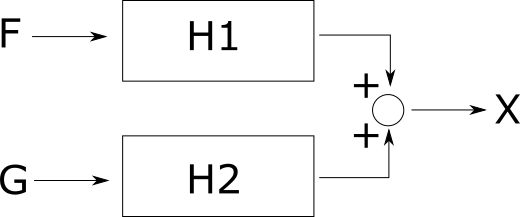
\includegraphics[width=\textwidth]{figures/problem3.png}
    \caption{Output of Listing 1}
    \label{}
  \end{figure}
  \newpage

  \section{}

  \subsection{Part A}

  Given,

  \[
      r = 0.01m, \quad h = 350 W/m^2C, \quad \rho = 7850, \quad c_p = 440J/kgC
    .\]

  \[
      k = 43W/m^2C, \quad T_f = 100C, \quad T_0 = 25C
    .\]

  Calculate Biot Criterion,

  \begin{equation}
    Bi = \frac{R_{cond}}{R_{conv}} = \frac{hL_c}{k}
  \end{equation}

  where,

  \begin{equation}
    L_c = \frac{V}{A} = \frac{r}{3} = 0.0033333
  \end{equation}

  The Biot Criterion is less than 0.1, therefore the temperature is spatially uniform.

  \subsection{Part B}

  Conservation of energy,

  \begin{equation}
    \frac{dU}{dt} = q_{in} - q_{out}
  \end{equation}

  where,

  \begin{equation}
    q_{in} = 0, \quad q_{out} = \frac{1}{R} (T - T_f), \quad \frac{dU}{dt} = \rho V c_p \dot T
  \end{equation}

  We can substitute these values to get the differential equation relating the temperature $ T $ to the temperature of the water $ T_f. $

  \begin{equation}
    mc_p \dot T = - \frac{1}{R} (T - T_f)
  \end{equation}

  which can be rewritten as,

  \begin{equation}
    R\rho V c_p \dot T + T = T_f
  \end{equation}

  \subsection{Part C}

  The time constant $ \tau $ is equal to,

  \begin{equation}
    \tau = R\rho V c_p = \frac{\rho V c_p}{h A_s} = \frac{7850 \cdot 440}{350} \cdot \frac{0.01}{3} = 32.89s
  \end{equation}

  \subsection{Part D}

  Treat the heating process as a step response. Take the laplace transform of both sides.

  \begin{equation}
    \frac{\rho V c_p}{h A_s} s T(s) + T(s) = \frac{T_f}{s}
  \end{equation}

  \begin{equation}
    T(s) = \ddfrac{T_f}{s\left( \ddfrac{\rho V c_p}{hA_s}s + 1 \right)}
  \end{equation}

  \begin{equation}
    T(s) = \frac{T_f}{s} - \frac{T_f}{s + \frac{hA_s}{\rho V c_p}}
  \end{equation}

  Take the inverse laplace transform

  \begin{equation}
    T(t) = T_f \left( 1 - e^{-\ddfrac{hA_s}{\rho V c_p}t} \right)
  \end{equation}

  \subsection{Part E}

  The result obtained in part b is modeled in simulink. The block diagram is shown in Figure \ref{fig:simulink} and the scope output is shown in Figure \ref{fig:scope}. As expected, we can see the of the sphere rise to the temperature of the water.

  \begin{figure}
    \centering
    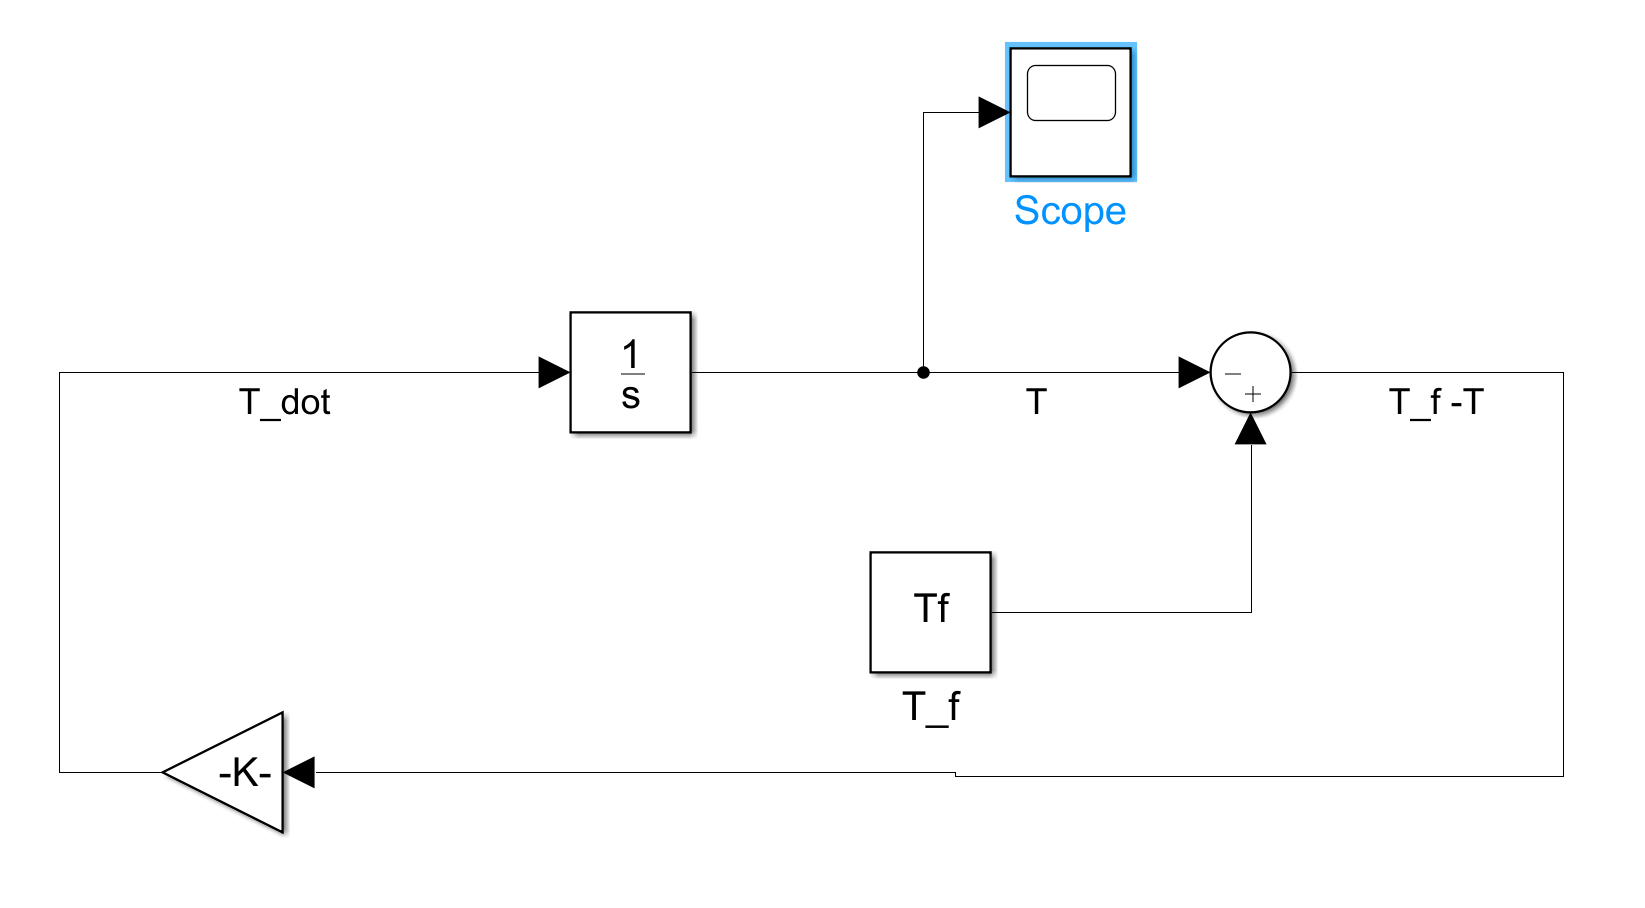
\includegraphics[width=\textwidth]{figures/simulink.png}
    \caption{Block diagram of result obtained in part b}
    \label{fig:simulink}
  \end{figure}

  \begin{figure}
    \centering
    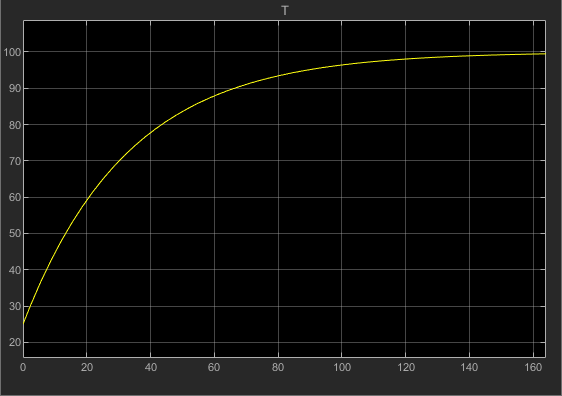
\includegraphics[width=\textwidth]{figures/scopesnip}
    \caption{Temperature as a function of time. Simulated for 164 seconds or 5 time constants.}
    \label{fig:scope}
  \end{figure}








\end{document}
